\documentclass{standalonex}
\usepackage{tikz}

\begin{document}
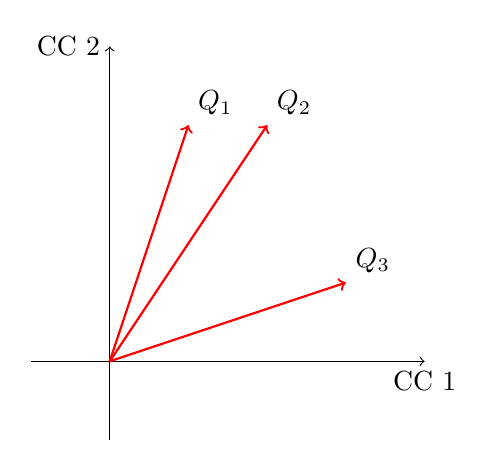
\begin{tikzpicture}
\draw[->] (-1,0) -- (4,0);
\draw node[below] at (4,0) {CC 1};
\draw[->] (0,-1) -- (0,4);
\draw node[left] at (0,4) {CC 2};
\draw[red,thick,->] (0,0) -- (1,3);
\draw node[above right] at (1,3) {$Q_1$};
\draw[red,thick,->] (0,0) -- (2,3);
\draw node[above right] at (2,3) {$Q_2$};
\draw[red,thick,->] (0,0) -- (3,1);
\draw node[above right] at (3,1) {$Q_3$};
\end{tikzpicture}
\end{document}
